\documentclass{standalone}
\usepackage{tikz}
\usepackage{ctex,siunitx}
\setCJKmainfont{Noto Serif CJK SC}
\usepackage{tkz-euclide}
\usepackage{amsmath}
\usetikzlibrary{patterns, calc,3d}
\usetikzlibrary {decorations.pathmorphing,decorations.pathreplacing,decorations.shapes}
\tikzset{label style/.append style={font=\small}}
\begin{document}
\small
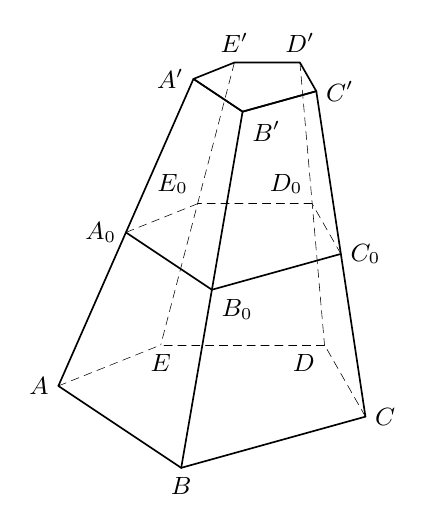
\begin{tikzpicture}[>=latex,scale=1.3]
  \useasboundingbox(-0.3,-1.1)rectangle(3.3,3.5);
  \tkzDefPoints{0/0/A,1.2/-0.8/B,3.0/-0.3/C,2.6/0.4/D,1.0/0.4/E,2.2/5/S}
  \tkzDefPointOnLine[pos=0.4](S,A)\tkzGetPoint{A'}
  \tkzDefPointOnLine[pos=0.4](S,B)\tkzGetPoint{B'}
  \tkzDefPointOnLine[pos=0.4](S,C)\tkzGetPoint{C'}
  \tkzDefPointOnLine[pos=0.4](S,D)\tkzGetPoint{D'}
  \tkzDefPointOnLine[pos=0.4](S,E)\tkzGetPoint{E'}
  \tkzDefPointOnLine[pos=0.7](S,A)\tkzGetPoint{A''}
  \tkzDefPointOnLine[pos=0.7](S,B)\tkzGetPoint{B''}
  \tkzDefPointOnLine[pos=0.7](S,C)\tkzGetPoint{C''}
  \tkzDefPointOnLine[pos=0.7](S,D)\tkzGetPoint{D''}
  \tkzDefPointOnLine[pos=0.7](S,E)\tkzGetPoint{E''}
  \tkzDrawSegments[semithick](A,B B,C A'',B'' B'',C'' A',B' B',C' A,A' B,B' C,C')
  \tkzDrawSegments[densely dashed](C,D D,E C'',D'' D'',E'' A,E  A'',E'' E',E D',D)
  \tkzDrawPolygon[semithick](A',B',C',D',E')
  \tkzLabelPoints[left](A,A')
  \tkzLabelPoints(B,E)
  \tkzLabelPoints[right](C,C')
  \tkzLabelPoints[below left](D)
  \tkzLabelPoints[below right](B')
  \tkzLabelPoints[above](E',D')
  \tkzLabelPoint[below right](B''){$B_0$}
  \tkzLabelPoint[left](A''){$A_0$}
  \tkzLabelPoint[right](C''){$C_0$}
  \tkzLabelPoint[above left](D''){$D_0$}
  \tkzLabelPoint[above left](E''){$E_0$}
\end{tikzpicture}
\end{document}